% Tormenta - report & viva notes (living document, updated every phase)
% Compile with pdflatex (e.g. on Overleaf). Upload this file together with
% reports/figures/*.png (either keep the ../reports/figures/ path or put the
% PNGs in a figures/ folder next to this file - both are searched).
\documentclass[11pt,a4paper]{article}

\usepackage[utf8]{inputenc}
\usepackage[T1]{fontenc}
\usepackage{lmodern}
\usepackage[margin=2.2cm]{geometry}
\usepackage{amsmath,amssymb}
\usepackage{booktabs,longtable,tabularx,array}
\usepackage{graphicx}
\usepackage{float}
\usepackage{caption}
\usepackage{enumitem}
\usepackage{xcolor}
\usepackage[colorlinks=true,linkcolor=blue!50!black,urlcolor=blue!50!black,citecolor=blue!50!black]{hyperref}

\graphicspath{{../reports/figures/}{figures/}}
\setlist{nosep,leftmargin=*}
\newcolumntype{L}{>{\raggedright\arraybackslash}X}
\newcommand{\code}[1]{\texttt{#1}}
\newcommand{\easy}[1]{\textit{In simple words:} #1}

\title{\textbf{Tormenta}\\[2pt]\large Nowcasting the Geomagnetic Kp Index from Solar-Wind Data\\[2pt]
\normalsize Report \& Viva Notes (living document)}
\author{Alizeh \and HRK\\[2pt]\small CT-378 Machine Learning, NED University of Engineering \& Technology, Fall 2026}
\date{Last updated: Phase 3 code complete (full training run pending)}

\begin{document}
\maketitle
\tableofcontents
\newpage

%=====================================================================
\section{Project overview}
%=====================================================================
\paragraph{Problem.} Estimate the current planetary geomagnetic activity index \textbf{Kp} (continuous, 0--9) from
upstream solar-wind and interplanetary magnetic field (IMF) measurements.

\paragraph{Task type.} Supervised \textbf{regression}. The target is continuous (Kp in steps of $1/3$), and
regression keeps the ordering information that a storm/no-storm classifier would throw away.

\paragraph{Framing: a nowcaster.} The model sees solar wind measured at the L1 Lagrange point, about
$1.5\times10^6$\,km sunward of Earth. At typical speeds (300--800\,km/s), that plasma reaches Earth
30--60 minutes later, so the model's effective horizon is about one hour. Multi-day forecasting would need
solar imagery and coronal mass ejection (CME) modelling, which is out of scope (future work).

\easy{a satellite between the Sun and Earth sees the ``space weather'' coming about an hour before it
arrives. We use those readings to say how disturbed Earth's magnetic field is right now.}

\paragraph{Why it matters.} Geomagnetic storms disturb GPS accuracy, HF radio, satellite drag and
electronics, and can induce currents in power grids and pipelines. Kp is the standard index operators use
(e.g.\ NOAA's G1--G5 storm scale).

\paragraph{Two non-negotiable design rules.}
\begin{enumerate}
\item \textbf{No target leakage.} Only solar causes are used as inputs. No geomagnetic index (Kp, ap, Ap, Dst,
AE, AL, AU, PCN) is ever a feature, and every feature at time $t$ uses only data at or before $t$.
\item \textbf{No train/serve skew.} Feature engineering is written once (\code{src/features.py}) and imported by
both the training pipeline and the live apps.
\end{enumerate}

%=====================================================================
\section{Physical background}
%=====================================================================
\subsection{Sun--Earth chain in brief}
\begin{enumerate}
\item The Sun's corona continuously expands into space as the \textbf{solar wind}, a hot, ionised gas
(mostly protons and electrons) at 250--1000\,km/s that carries the Sun's magnetic field with it (the
\textbf{IMF}).
\item Earth's magnetic field carves out a cavity, the \textbf{magnetosphere}. Its sunward boundary sits about
10 Earth radii away, preceded by a \textbf{bow shock}.
\item When the IMF points \textbf{southward} (negative $B_z$), it is anti-parallel to Earth's field at the dayside
boundary. The fields \textbf{reconnect} and solar-wind energy pours into the magnetosphere. This drives storms.
Northward IMF largely shields Earth.
\item The energy input rate scales roughly with $V\cdot B_s$ (speed times southward field), which is the
solar-wind \textbf{electric field}. Fast wind with strong southward field gives the biggest storms.
\item The resulting currents disturb ground magnetometers, and \textbf{Kp} summarises that disturbance.
\end{enumerate}
\easy{the solar wind is like a wind carrying a magnet. If its magnet points the ``wrong'' way (south), it
locks onto Earth's magnet and pumps energy in, and Earth's magnetic field starts shaking.}

\subsection{Coordinate system: GSM}
IMF components are given in \textbf{Geocentric Solar Magnetospheric (GSM)} coordinates:
\begin{itemize}
\item $X$ points from Earth to the Sun.
\item $Z$ is the projection of Earth's magnetic dipole axis onto the plane perpendicular to $X$.
\item $Y$ completes the right-handed set.
\end{itemize}
GSM is the natural frame for coupling, because $B_z^{\rm GSM}<0$ means ``anti-parallel to Earth's dipole''.
\easy{GSM is a set of axes tilted to line up with Earth's magnet, so ``negative $B_z$'' directly means
``pointing against Earth's magnet''.}

\subsection{The Kp index}
\begin{itemize}
\item Derived by GFZ Potsdam from the 3-hourly range of horizontal magnetic disturbance at 13 subauroral
observatories. Each local value (the K index) is quasi-logarithmic, and Kp is a standardised planetary average.
\item 28 discrete values per 3-hour UT block (00--03, 03--06, \dots, 21--24 UT):
0o, 0+, 1$-$, 1o, 1+, \dots, 9$-$, 9o. In decimal form these are $0, 0.333, 0.667, 1, \dots, 9$.
\item The scale is quasi-logarithmic: one Kp step is roughly a doubling of the disturbance amplitude.
\end{itemize}
\easy{Kp is a 0--9 ``earthquake scale'' for Earth's magnetic field, updated every 3 hours.}

\begin{table}[H]\centering\small
\caption{NOAA geomagnetic storm scale. Kp is rounded to the nearest integer, so 5$-$ (4.67) already counts as G1.
Our bin edges therefore sit at the half-integers (3.5, 4.5, 5.5, 6.5).}
\begin{tabular}{llll}\toprule
Kp & NOAA level & Description & Our bin label\\\midrule
0--3 & -- & quiet to unsettled & \code{0-3}\\
4 & -- & active & \code{4}\\
5 & G1 & minor storm & \code{5 (G1)}\\
6 & G2 & moderate storm & \code{6 (G2)}\\
7 & G3 & strong storm & \code{7+ (G3-G5)}\\
8 & G4 & severe storm & \code{7+ (G3-G5)}\\
9 & G5 & extreme storm & \code{7+ (G3-G5)}\\\bottomrule
\end{tabular}\end{table}

\subsection{F10.7 solar radio flux}
F10.7 is the solar radio emission at 10.7\,cm (2800\,MHz), measured daily around 20\,UT at Penticton, Canada, in
solar flux units (1\,sfu $=10^{-22}$\,W\,m$^{-2}$\,Hz$^{-1}$). It is a standard proxy for overall solar
activity and tracks the 11-year solar cycle.
\easy{a daily ``how active is the Sun overall'' number. It changes slowly over the 11-year cycle, so it gives
background context rather than predicting individual storms.}

%=====================================================================
\section{Data sources}
%=====================================================================
\begin{table}[H]\centering\small
\caption{Data sources used in Tormenta.}
\begin{tabularx}{\textwidth}{p{2.2cm}LLp{2.4cm}}\toprule
Source & Content \& role & Access & Licence\\\midrule
NASA OMNI2 hourly (GSFC SPDF) &
Features (training). Hourly solar-wind plasma and IMF, cross-calibrated from ACE, Wind and other spacecraft and
time-shifted to Earth's bow-shock nose. Seed file: 1998-01-01 to 2026-01-10, 245{,}688 rows. Lags real time by
months. &
OMNIWeb subset (\code{.lst}+\code{.fmt}); retrain loop: \url{https://spdf.gsfc.nasa.gov/pub/data/omni/low_res_omni/} &
NASA open data\\\addlinespace
GFZ Potsdam Kp &
Target (label). Definitive Kp since 1932, daily rows with 8 three-hourly values, a definitive flag $D$, and
observed and adjusted F10.7. &
\url{https://kp.gfz.de} &
CC BY 4.0 (sunspot numbers CC BY-NC, not used)\\\addlinespace
NOAA SWPC real-time &
Features (live serving only). Real-time L1 IMF and plasma (DSCOVR/ACE), estimated Kp for comparison, daily
F10.7. &
\url{https://services.swpc.noaa.gov} (JSON, no authentication) &
US Government public domain\\\bottomrule
\end{tabularx}\end{table}

\paragraph{Two-tier design.} OMNI is definitive but delayed, so it is used for (re)training. SWPC is real-time
but raw, so it is used for live inference. The archive and the live feed differ in two documented ways:
\begin{itemize}
\item \textbf{Cadence:} OMNI is hourly and SWPC is 1--5 min. Live data is resampled to hourly means before
feature engineering.
\item \textbf{Propagation:} OMNI is time-shifted to the bow-shock nose, while SWPC is at L1. We accept this
$\sim$30--60 min offset as the nowcast horizon.
\end{itemize}

\paragraph{Suggested data acknowledgements for the report.}
``We acknowledge use of NASA/GSFC's Space Physics Data Facility's OMNIWeb service and OMNI data''
\cite{king2005}. ``Kp index provided by GFZ German Research Centre for Geosciences'' \cite{matzka2021}.
Real-time data courtesy of NOAA Space Weather Prediction Center.

%=====================================================================
\section{Variable glossary}
%=====================================================================
\begin{longtable}{p{2.4cm}p{1.4cm}p{5.6cm}p{5.6cm}}
\caption{Variables in the processed dataset and planned derived features.}\\\toprule
Name in code & Unit & Technical meaning & In simple words\\\midrule\endfirsthead
\toprule Name in code & Unit & Technical meaning & In simple words\\\midrule\endhead
\multicolumn{4}{l}{\textbf{Raw inputs (from OMNI; reconstructable from SWPC live)}}\\
\code{b\_scalar} & nT & Hourly mean of the IMF magnitude $|\mathbf{B}|$ & How strong the Sun's magnetic field is when it reaches us\\
\code{bx} & nT & IMF $X$ component (GSE = GSM for $X$) & Field along the Sun--Earth line; weak effect on storms\\
\code{by\_gsm} & nT & IMF $Y$ component, GSM & Sideways field; matters through the clock angle\\
\code{bz\_gsm} & nT & IMF $Z$ component, GSM; negative = southward & \textbf{The key variable}: negative (south) means energy gets in\\
\code{temperature} & K & Proton temperature & How hot the wind is; hot usually means fast\\
\code{density} & cm$^{-3}$ & Proton number density & How many particles per cubic centimetre\\
\code{speed} & km/s & Bulk flow speed & How fast the wind blows\\
\code{f107\_obs} & sfu & Observed 10.7\,cm solar radio flux (GFZ/Penticton), daily & Overall solar activity level\\\addlinespace
\multicolumn{4}{l}{\textbf{Target and flags}}\\
\code{kp} & -- & Kp of the 3-h UT block containing the hour & The answer the model must predict\\
\code{kp\_definitive} & bool & GFZ flag $D=2$ (final). Only these rows are trained on & Whether the Kp value is final\\\addlinespace
\multicolumn{4}{l}{\textbf{OMNI precomputed (validation only, never features)}}\\
\code{omni\_pressure} & nPa & Flow pressure (OMNI includes an alpha-particle factor) & Recomputed by us instead\\
\code{omni\_efield} & mV/m & $-V B_z\times10^{-3}$ & Recomputed by us instead\\
\code{omni\_beta} & -- & Plasma beta & Recomputed by us instead\\
\code{omni\_mach\_a}, \code{omni\_mach\_ms} & -- & Alfv\'en / magnetosonic Mach numbers & Recomputed by us instead\\\addlinespace
\multicolumn{4}{l}{\textbf{Derived features (Phase 3, \code{features.py}, same code for training and live)}}\\
$P$ & nPa & $P=1.6726\times10^{-6}\,N V^2$ (protons only) & How hard the wind pushes on Earth's field\\
$E$ & mV/m & $E=-V B_z\times10^{-3}$ & Rate at which energy is delivered\\
$V B_s$ & mV/m & $V\max(-B_z,0)\times10^{-3}$ (rectified $E$) & Only the southward part counts\\
$\beta$ & -- & $(4.16\times10^{-5}T+5.34)\,N/B^2$ & Gas pressure vs magnetic pressure\\
$M_A$ & -- & $V\sqrt{N}/(20B)$ & Wind speed relative to magnetic wave speed\\
$B_T$, $\theta$ & nT, rad & $B_T=\sqrt{B_y^2+B_z^2}$, $\theta=\operatorname{atan2}(B_y,B_z)$ & Field strength and direction across the flow\\
Newell coupling & -- & $V^{4/3}B_T^{2/3}\sin^{8/3}(\theta/2)$ \cite{newell2007} & Best-known single formula for ``how much energy gets in''\\
Lags (16) & -- & $B_z, V, N, VB_s$ at $t-1, 3, 6, 9$\,h & What the wind was doing a few hours ago\\
Rolling stats (19) & -- & Trailing mean/std of $B_z$ and $V$ over 3/6/9\,h; mean Newell coupling over 3/6/9\,h; min $B_z$ and max $V$ over 3\,h; mean $V$ over 12/24\,h & Recent average, variability and extremes\\
F10.7 features (2) & sfu & Previous day's value; trailing 81-day mean. Days $>2\times$ the trailing 27-day median are treated as flare-contaminated (missing) & Solar background without peeking at the future\\
Cyclical time & -- & $\sin/\cos$ of hour-of-day and day-of-year & Time of day and season, as circles not lines\\\bottomrule
\end{longtable}

%=====================================================================
\section{System architecture}
%=====================================================================
\begin{itemize}
\item \textbf{Fast loop} (minutes, inference only): SWPC feeds $\rightarrow$ hourly resample $\rightarrow$
\code{features.py} $\rightarrow$ model $\rightarrow$ predicted Kp with interval, compared against SWPC estimated Kp.
\item \textbf{Slow loop} (weekly, GitHub Actions): fetch OMNI and GFZ $\rightarrow$ rebuild $\rightarrow$ retrain
$\rightarrow$ validation gate $\rightarrow$ promote $\rightarrow$ redeploy.
\item \textbf{Validation gate:} both the incumbent and the candidate are scored, in the same run, on the latest
6 months of definitive labels, which neither model was trained on. The candidate is promoted only if its RMSE
is at most $1.02\times$ the incumbent's.
\item \textbf{Deployments:} Streamlit Community Cloud (dashboard), Hugging Face Space (Gradio demo and model card),
Flask (REST API, localhost). All three load the same model with the same pinned scikit-learn.
\end{itemize}

%=====================================================================
\section{Implementation log}
%=====================================================================
Each entry covers \textbf{what} the file does, \textbf{how}, \textbf{why}, and \textbf{what we got}.

\subsection{Phase 0: setup}
\paragraph{\code{src/config.py}.}
\begin{itemize}
\item \textit{What:} the single source of every path, column name and constant.
\item \textit{Why:} the training code and the live apps cannot drift apart if constants live in one place.
\item \textit{Result:} OMNI fill sentinels (999.9, 9999999., 9999., 99.99, \dots) were verified against the
actual file maxima. Storm bins follow NOAA rounding. F10.7 is taken from GFZ's observed value, the same quantity
SWPC serves live.
\end{itemize}

\paragraph{\code{requirements.txt}.}
\begin{itemize}
\item \textit{What:} exact package pins (scikit-learn 1.9.1, pandas 3.1.0, numpy 2.5.4, \dots), Python 3.12.
\item \textit{Why:} joblib-pickled models can fail or behave differently across scikit-learn versions. Python
3.12 is Streamlit Cloud's default and is supported by Hugging Face Spaces and GitHub Actions; 3.14 had reported
deployment issues.
\end{itemize}

\subsection{Phase 1: ingestion and preprocessing}
\paragraph{\code{src/ingest/fetch\_omni.py}.}
\begin{itemize}
\item \textit{What:} parses the OMNIWeb subset.
\item \textit{How:} replaces fill sentinels with NaN \emph{per column}, then builds a UTC timestamp from
year + day-of-year + hour.
\item \textit{Result:} 245{,}688 hourly rows, 1998-01-01 to 2026-01-10.
\end{itemize}

\paragraph{\code{src/ingest/fetch\_gfz.py}.}
\begin{itemize}
\item \textit{What:} reads the GFZ Kp file.
\item \textit{How:} melts Kp1--Kp8 into a 3-hourly series stamped at block start (00, 03, \dots, 21\,UT), and
keeps the definitive flag and the observed F10.7.
\end{itemize}

\paragraph{\code{src/preprocessing.py}.}
\begin{itemize}
\item \textit{What:} builds the hourly modelling table.
\item \textit{How:}
  \begin{enumerate}
  \item Reindexes to a \textbf{complete hourly grid}, so later shift and rolling operations never jump across
  data gaps.
  \item Labels each hour $h$ with the Kp of the block containing $h$ (block start $=3\lfloor h/3\rfloor$).
  \item Attaches the daily F10.7.
  \item Runs sanity checks: unique timestamps, no grid holes, Kp $\in[0,9]$.
  \end{enumerate}
\item \textit{Why hourly, not 3-hourly:} averaging each 3-h block would use solar wind from the whole block,
which a live system mid-block cannot have. That is a subtle form of train/serve skew. The hourly design with
trailing windows matches live use exactly.
\item \textit{Result:} 245{,}688 rows and 15 columns.
  \begin{itemize}
  \item All labels are definitive. That is about 81{,}900 \emph{independent} 3-h labels, because three
  consecutive rows share one Kp value; we never claim $n=245$k independent samples.
  \item Maximum missingness per column is 2.3\% (density, temperature); $B_z$ is 0.16\%.
  \end{itemize}
\item \textit{Deliberately deferred:}
  \begin{itemize}
  \item Imputation and scaling go inside the scikit-learn \code{Pipeline}, fitted on training years only, to
  avoid leakage.
  \item Derived features go in \code{features.py}, so the live apps use identical code.
  \end{itemize}
\end{itemize}

\subsection{Phase 3: features and modelling}
\paragraph{\code{src/features.py} (shared by training and serving).}
\begin{itemize}
\item \textit{What:} builds 56 features in six groups: raw (7), derived physics (8), lags (16), trailing rolling
statistics (19), F10.7 (2) and cyclical time (4); see the glossary.
\item \textit{How:} one pure function, \code{build\_features(hourly, f107\_daily)}.
  \begin{itemize}
  \item It first enforces a complete hourly grid (\code{asfreq("h")}).
  \item All windows are trailing, so every feature at $t$ uses data at or before $t$.
  \end{itemize}
\item \textit{Why:}
  \begin{itemize}
  \item A single implementation removes train/serve skew.
  \item The 12/24\,h speed means follow the lag-correlation result (speed retains memory for about a day).
  \item The previous-day F10.7 respects its $\sim$20\,UT measurement time.
  \item The cyclical time features let the model capture the semi-annual/diurnal modulation of coupling by
  the dipole tilt (Russell--McPherron effect).
  \end{itemize}
\item \textit{Verification against OMNI:} on 2005--2006, our $E$, $\beta$ and $M_A$ equal OMNI's columns
(median ratio 1.000, $r=1.000$). Our proton-only pressure is $0.88\times$ OMNI's ($r=0.989$), a near-constant
factor from the alpha-particle term that is deliberately omitted because SWPC provides no alpha data.
\end{itemize}

\paragraph{\code{tests/test\_features.py}.} Four automated tests:
\begin{enumerate}
\item \textbf{Causality:} features at $t$ are unchanged when later rows are appended.
\item \textbf{Gaps:} dropped rows become NaN rows, so lags never cross gaps.
\item \textbf{F10.7:} flare spikes are removed and only the previous day's value is used.
\item \textbf{Inputs:} no geomagnetic index is used, and there are more than 15 features.
\end{enumerate}
These tests turn the two silent failure modes (future leakage and gap-crossing lags) into automatic checks.

\paragraph{\code{src/train.py}.}
\begin{itemize}
\item \textbf{Baselines:}
  \begin{itemize}
  \item Persistence: Kp of the previous 3-h block. It uses past Kp, so it is a baseline only, never a feature.
  \item Linear Regression.
  \end{itemize}
\item \textbf{Model families:} KNN, SVR (RBF kernel), Random Forest, HistGradientBoosting. Linear, KNN and SVR
use median imputation and standard scaling inside a \code{Pipeline}.
\item \textbf{Tuning:} \code{RandomizedSearchCV} with \code{TimeSeriesSplit(5)} on the training years (each
fold trains on the past and validates on the future), scored by RMSE.
  \begin{itemize}
  \item KNN and SVR are tuned and fitted on a strided subsample (every 9th hour, $\approx$18.5k rows).
  \item Random Forest is tuned on every 3rd hour and refit on all hours.
  \end{itemize}
\item \textbf{Selection and fitting diagnosis:} the validation table reports validation RMSE/MAE/$R^2$, storm-hour
RMSE, CV RMSE and training RMSE. A large train--CV gap indicates overfitting; uniformly high errors indicate
underfitting. Because validation is at solar minimum, CV, validation and storm metrics are read together.
\item \textbf{Test:} every family is refit on train+val with its tuned parameters and evaluated once on
2020--2026.
\item \textbf{Ablation:} HistGB with sample weights $w=1+\text{Kp}/3$ vs unweighted.
\item \textbf{Prediction interval:} two quantile HistGBs ($q=0.1, 0.9$) give a nominal 80\% interval. It is
widened to always contain the point estimate, and its empirical coverage is reported.
\item \textbf{Production model:} HistGB (point + quantiles) trained on all definitive data up to the start of the
last 6 months, which serve as the validation-gate holdout of the weekly retrain. It is saved with its feature
list, parameters and scikit-learn version.
\end{itemize}

\paragraph{\code{src/evaluate.py}, \code{src/predict.py}.}
\begin{itemize}
\item \code{evaluate.py}: metrics (including storm-only RMSE/MAE), error and bias by storm level,
predicted-vs-observed hexbins, permutation importance, storm case-study plot.
\item \code{predict.py}: loads the bundle and returns Kp with its interval, clipped to $[0,9]$.
\end{itemize}

\paragraph{Results.} \textit{Pending the full training run of \code{03\_modeling.ipynb}.} A fast smoke test
(tiny search, heavy subsampling) already showed:
\begin{itemize}
\item HistGB beating persistence by about 27\% in test RMSE.
\item Systematic under-prediction of G3+ hours.
\item Interval coverage below the nominal 80\%.
\end{itemize}
These will be confirmed or revised with the full run.

%=====================================================================
\section{Exploratory data analysis (Phase 2)}
%=====================================================================
All relationships used for modelling decisions are computed on the \textbf{training years (1998--2016)} only;
plots involving later years are descriptive. Notebook: \code{notebooks/02\_eda.ipynb}.

\subsection{Target distribution and storm rarity}
\begin{figure}[H]\centering
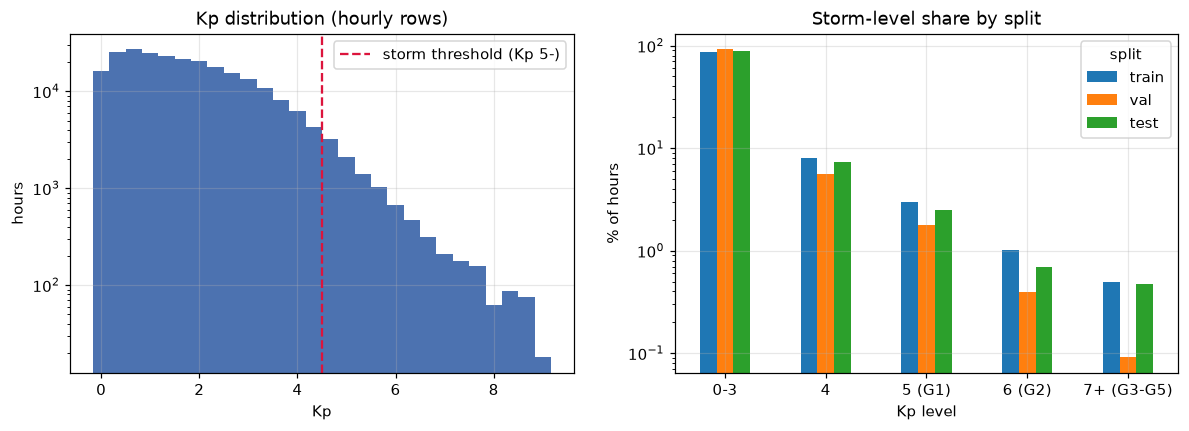
\includegraphics[width=\textwidth]{01_kp_distribution.png}
\caption{Left: distribution of hourly Kp (log scale); the dashed line is the storm threshold Kp\,=\,5$-$.
Right: share of hours per storm level in each split (log scale).}
\end{figure}
\begin{itemize}
\item Kp is strongly right-skewed. Storms (Kp $\geq$ 5$-$) make up only \textbf{4.06\%} of hours, and G3+ storms
about \textbf{0.5\%}.
\item By split, G3+ hours are 0.50\% (train), \textbf{0.09\%} (validation) and 0.47\% (test).
\item \textit{Implications:}
  \begin{itemize}
  \item A squared-error model will be pulled toward quiet values and under-predict storms. We will report
  error by storm level and run a sample-weighting ablation ($w=1+\text{Kp}/3$).
  \item The \textbf{validation years 2017--2019 fall at solar minimum}, so validation alone is a weak judge of
  storm performance. Model selection should also consider cross-validation scores and storm-level errors.
\end{itemize}
\end{itemize}
\easy{big storms are rare, so a lazy model could just always guess ``quiet'' and still look decent on
average. We must check how it does on storms specifically.}

\subsection{Input distributions}
\begin{figure}[H]\centering
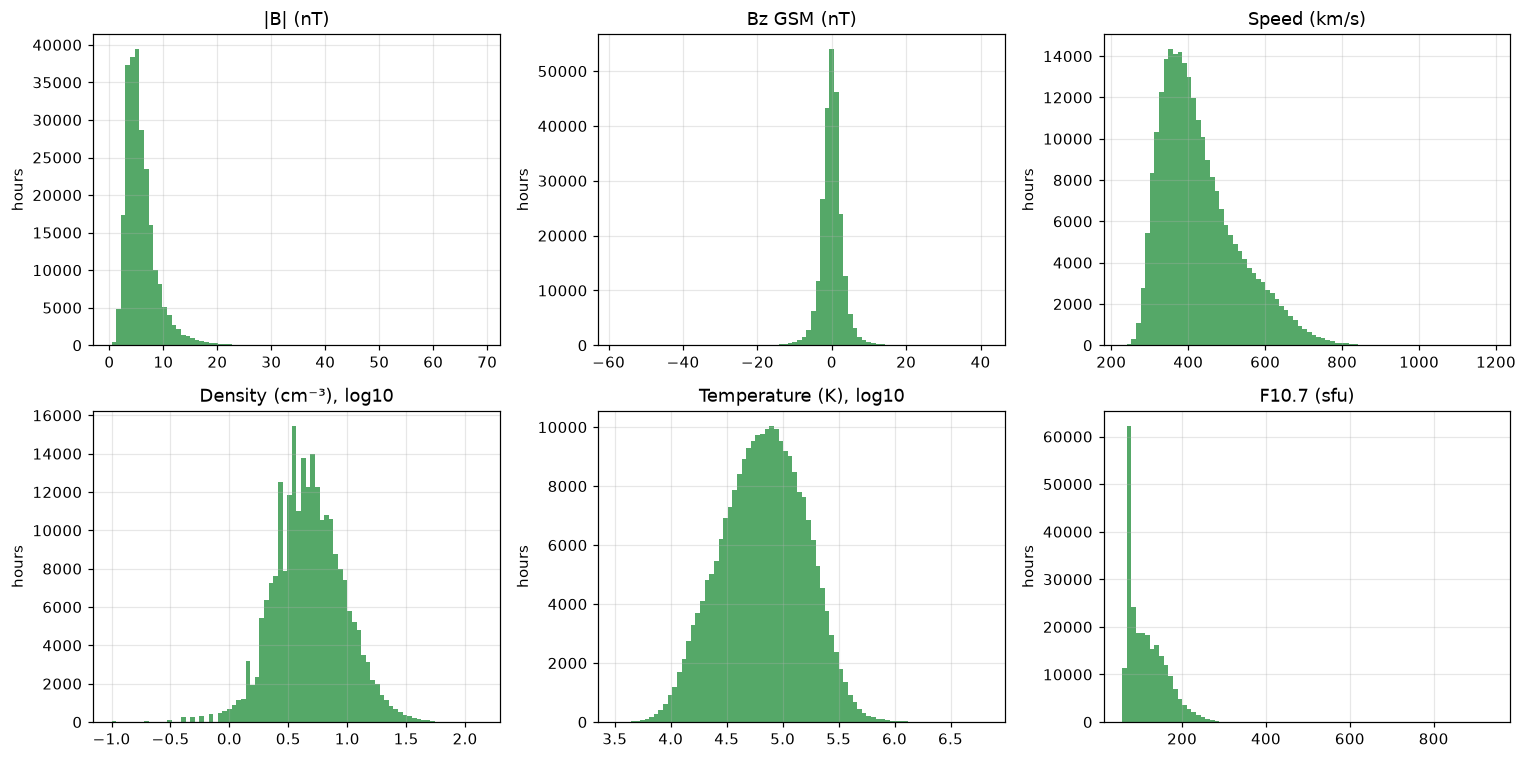
\includegraphics[width=\textwidth]{02_input_distributions.png}
\caption{Distributions of the main inputs. Density and temperature are shown as $\log_{10}$.}
\end{figure}
\begin{itemize}
\item $B_z$ is centred at 0 nT ($\sigma\approx3$\,nT) with long tails (min $-57.8$, max 41.6\,nT).
\item Speed is right-skewed (median 407\,km/s, max 1189\,km/s).
\item Density and temperature are approximately log-normal.
\item F10.7 is bimodal, reflecting solar minimum and maximum years.
\item \textit{Implication:} tree models are insensitive to skew, but KNN and SVR need scaling (and possibly
log-transformed density and temperature).
\end{itemize}

\subsection{Missing data}
\begin{figure}[H]\centering
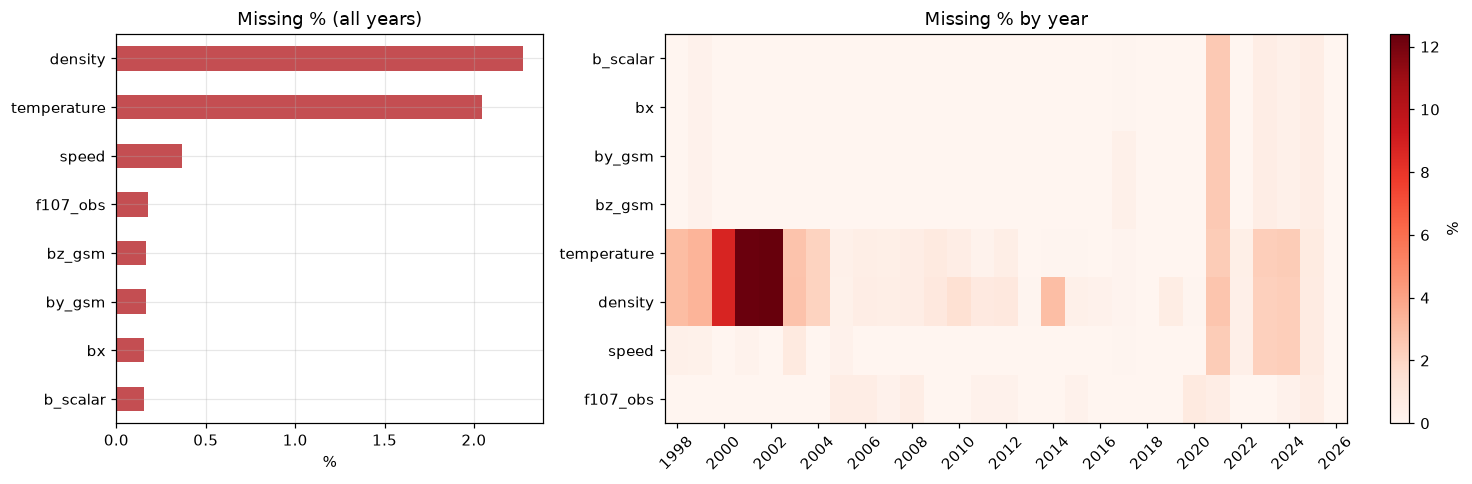
\includegraphics[width=\textwidth]{03_missingness.png}
\caption{Left: overall missing share per input. Right: missing share by year.}
\end{figure}
\begin{itemize}
\item Plasma moments (density, temperature) are the least complete, about 2\% overall and up to
$\sim$12\% in 2000--2002, consistent with known ACE/SWEPAM data issues in that period. All fields show a gap in
2021.
\item Gap lengths: half of the density gaps are $\leq$3\,h, but \textbf{52\% of missing density hours lie in gaps
longer than 24\,h} (longest 104\,h). $B_z$ has only 51 gaps.
\item \textit{Implication:}
  \begin{itemize}
  \item Short-gap interpolation cannot cover the long outages.
  \item HistGradientBoosting handles NaN natively, which suits the production model.
  \item The other models get median imputation inside the pipeline, fitted on training years only.
  \end{itemize}
\end{itemize}
\easy{sometimes the satellite's instruments go quiet for days. We can't just ``connect the dots'' over
such long gaps, so we use a model that can cope with blanks.}

\subsection{Physical drivers of Kp}
\begin{figure}[H]\centering
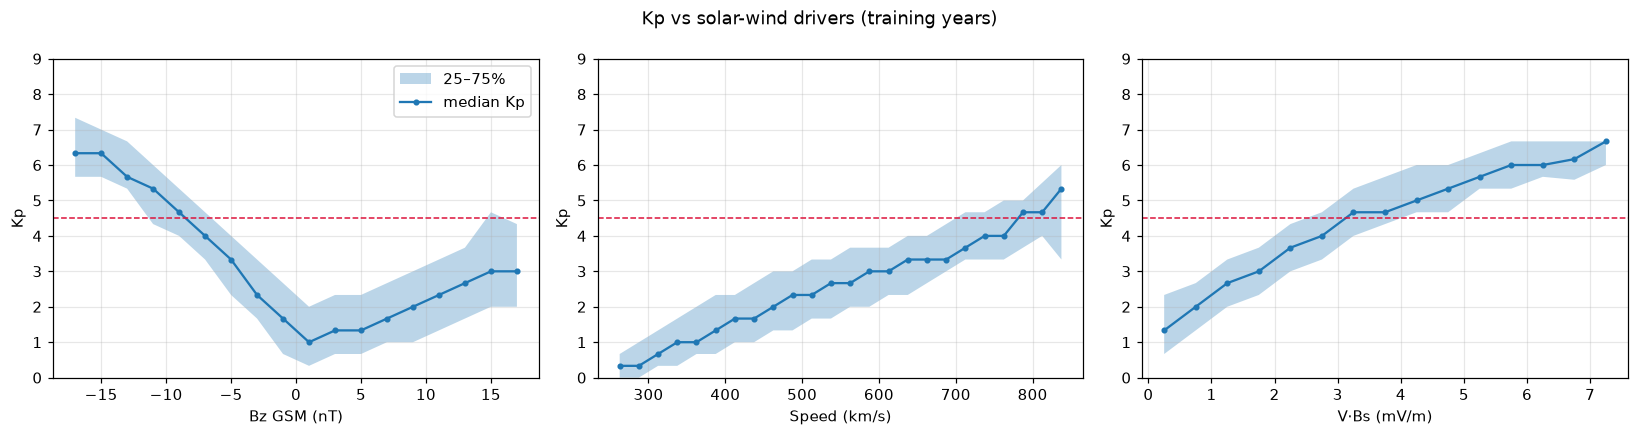
\includegraphics[width=\textwidth]{04_kp_vs_drivers.png}
\caption{Median Kp (line) and inter-quartile range (band) versus binned $B_z$, speed and $V B_s$ (training
years; bins with $\geq$50 hours).}
\end{figure}
\begin{itemize}
\item Kp increases monotonically as $B_z$ becomes more negative: the median crosses storm level near
$B_z\approx-9$\,nT and reaches $\sim$6.3 at $-17$\,nT.
\item Northward $B_z$ raises Kp much less. The asymmetry is the signature of dayside reconnection.
\item Kp rises nearly linearly with speed, and the median reaches storm level above about 780\,km/s.
\item $V B_s$ gives the cleanest monotonic relation: the median crosses storm level near 3.2\,mV/m.
\end{itemize}
\easy{the plot confirms the physics: south-pointing field plus fast wind means storms.}

\begin{figure}[H]\centering
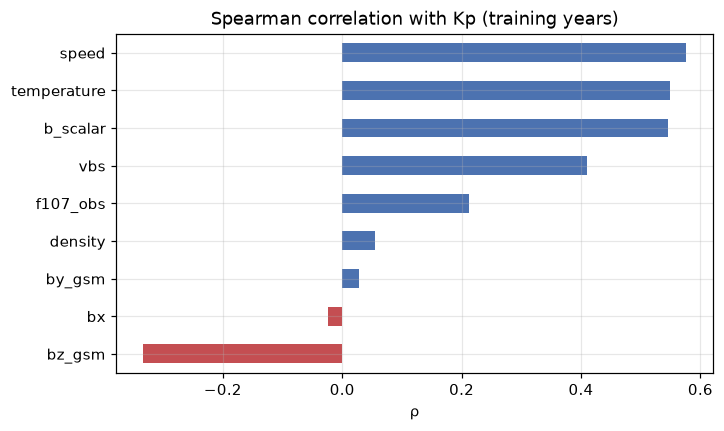
\includegraphics[width=0.65\textwidth]{05_correlation.png}
\caption{Spearman rank correlation of each input with Kp (training years).}
\end{figure}
\begin{itemize}
\item Spearman $\rho$: speed 0.58, temperature 0.55, $|B|$ 0.55, $V B_s$ 0.41, $B_z$ $-0.33$, F10.7 0.21.
$B_x$, $B_y$ and density are close to 0.
\item Temperature correlates with Kp largely because hot wind is fast wind (the two are physically linked).
\item $B_y$ is weak on its own but enters through the clock angle and Newell coupling.
\item Spearman (rank) correlation is used because the relations are monotonic but non-linear.
\end{itemize}

\subsection{Time delay}
\begin{figure}[H]\centering
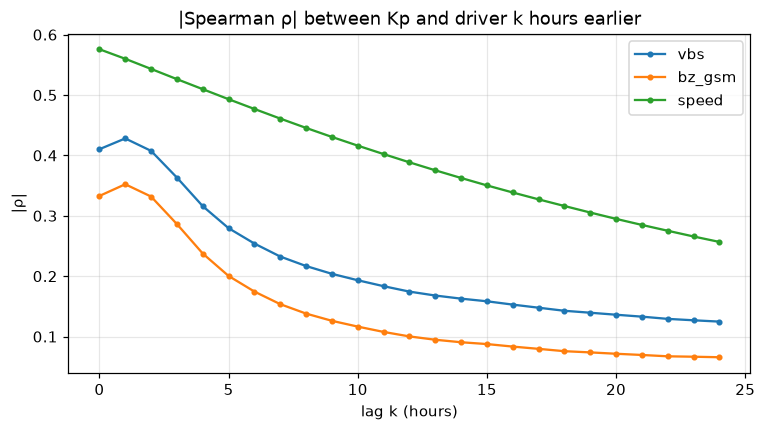
\includegraphics[width=0.75\textwidth]{06_lag_correlation.png}
\caption{Absolute Spearman correlation between Kp and each driver measured $k$ hours earlier (training years).}
\end{figure}
\begin{itemize}
\item $V B_s$ correlates best \textbf{1\,h earlier} ($\rho=0.43$ vs 0.41 at lag 0), consistent with
magnetospheric response time. It decays to 0.25 at 6\,h and 0.20 at 9\,h.
\item Speed keeps memory far longer ($\rho=0.26$ at 24\,h): fast streams last for days.
\item \textit{Implication:}
  \begin{itemize}
  \item This justifies the 1/3/6/9\,h lags and the trailing windows.
  \item It suggests adding 12--24\,h trailing speed means. That requires $\geq$33\,h of live history, so the live
  app would use SWPC's 3-day products.
  \end{itemize}
\end{itemize}
\easy{Earth reacts to the solar wind with about an hour's delay, and a fast wind stream keeps things stirred up
for a day. So the model should also see the recent past, not just the current hour.}

\subsection{Solar cycle and data split}
\begin{figure}[H]\centering
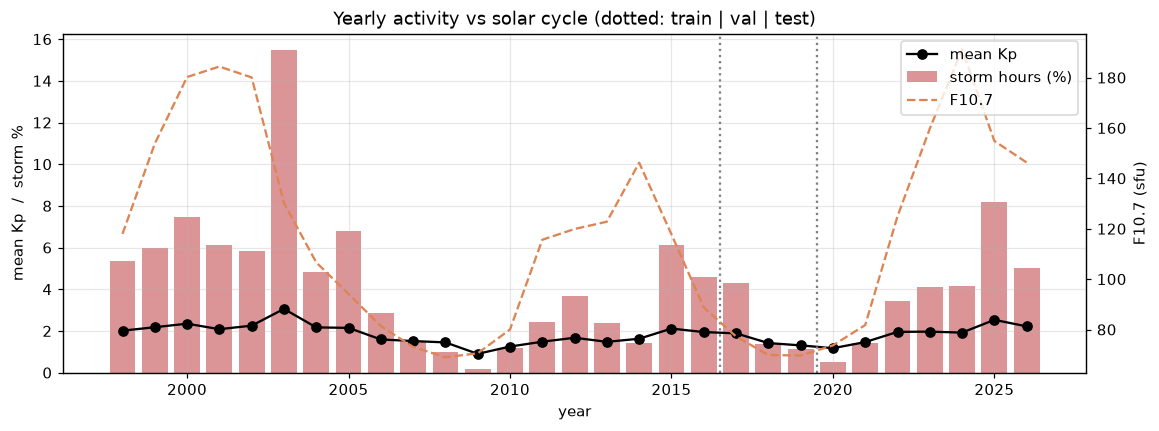
\includegraphics[width=\textwidth]{07_solar_cycle.png}
\caption{Yearly mean Kp, share of storm hours, and mean F10.7. Dotted lines separate train | validation | test.}
\end{figure}
\begin{itemize}
\item Activity follows the $\sim$11-year cycle, with cycle 23 peaking around 2000--2003. The year 2003 (Halloween
storms) has 15.5\% storm hours, while 2009 and 2020 are the quietest (0.2\% and 0.5\%).
\item The training set spans cycle 23 and most of cycle 24. The test set covers the rise and maximum of cycle 25,
including 2024--2025.
\item A time-ordered split is essential: shuffled splits would put hours from the same storm on both sides,
because neighbouring hours are highly correlated.
\end{itemize}

\subsection{Case study: the May 2024 (Gannon) storm}
\begin{figure}[H]\centering
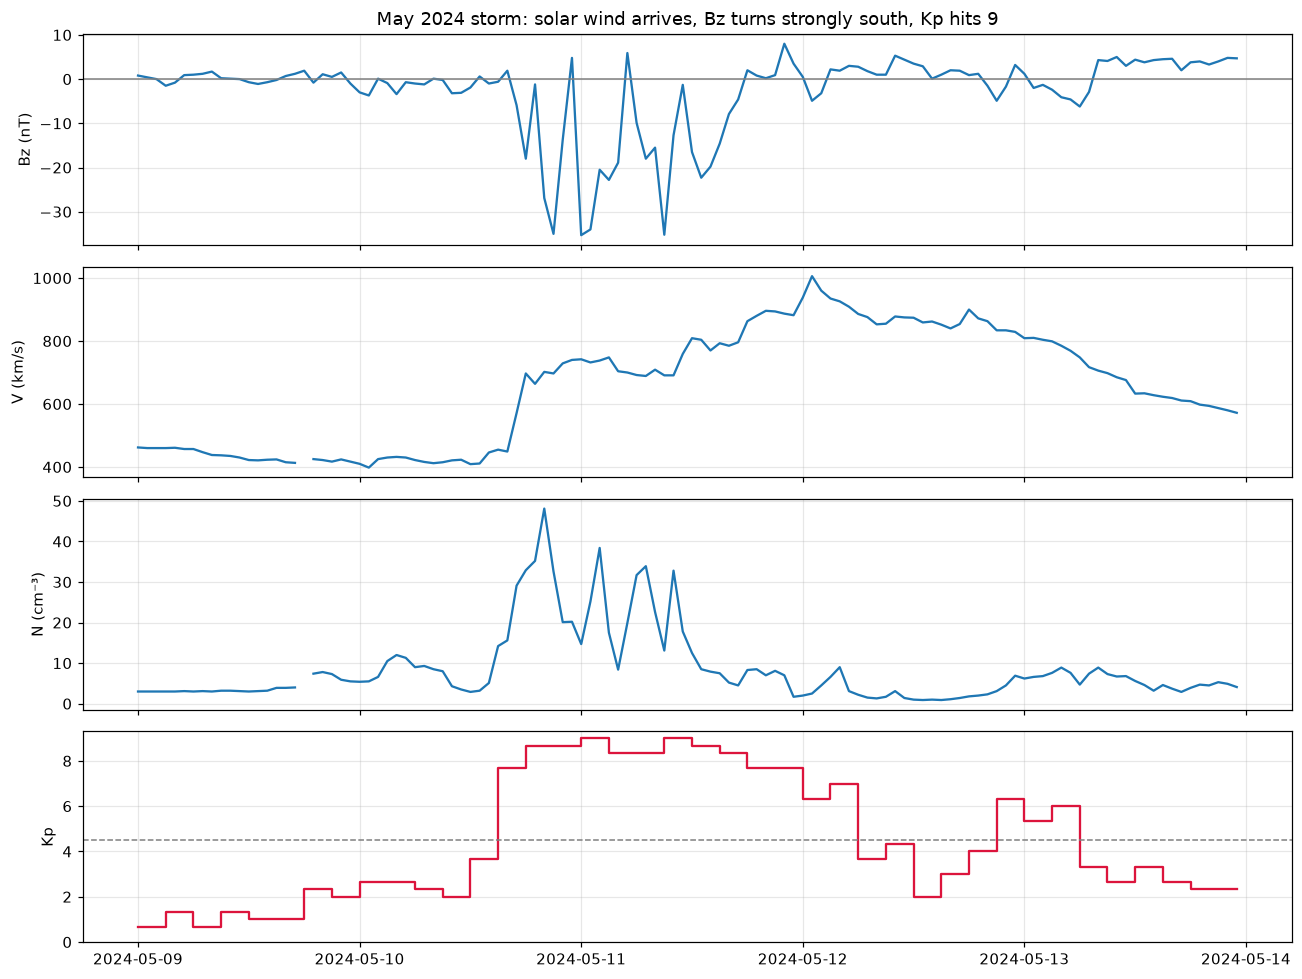
\includegraphics[width=\textwidth]{08_may2024_storm.png}
\caption{10--11 May 2024: $B_z$, speed, density and Kp. The storm is in the held-out test set.}
\end{figure}
\begin{itemize}
\item On 10 May around 17\,UT a CME shock arrives. Speed jumps from $\sim$450 to 700+\,km/s and density spikes
to $\sim$48\,cm$^{-3}$.
\item $B_z$ then swings repeatedly to about $-35$\,nT, and Kp climbs to 9 (G5) for several blocks, the strongest
storm in two decades.
\item It lies in the test set, so it is an honest test of extreme-event generalisation. Under-prediction at
Kp 8--9 is expected and will be discussed.
\end{itemize}

\subsection{Extreme values: errors or physics?}
\begin{table}[H]\centering\small
\caption{Share of extreme-value hours that occur during storms (baseline: 4.1\% of all hours are storm hours).}
\begin{tabular}{lrr}\toprule
Condition & Hours & \% during storms\\\midrule
$|B_z|>30$\,nT & 46 & 87.0\\
speed $>900$\,km/s & 140 & 92.1\\
density $>50$\,cm$^{-3}$ & 135 & 31.9\\
temperature $>10^6$\,K & 167 & 51.5\\\bottomrule
\end{tabular}\end{table}
\begin{itemize}
\item Extreme values cluster overwhelmingly in storms (8--22$\times$ the baseline rate), so they are
\textbf{real physics, not sensor errors}, and are kept.
\item The exception is F10.7: 7 daily values exceed 400\,sfu (max 938.6 on 2011-03-07). These are isolated
one-day spikes caused by solar flares contaminating the noon measurement, and they will be cleaned in Phase 3
(e.g.\ by flagging values far above the trailing median).
\end{itemize}

%=====================================================================
\section{Key design decisions (for the viva)}
%=====================================================================
\begin{longtable}{p{4.6cm}p{11.2cm}}\toprule
Decision & Reason\\\midrule\endhead
Regression, not classification & Kp is ordinal and continuous; regression keeps the full information. Storm/no-storm can be derived by thresholding.\\
No geomagnetic indices as inputs & Same-time indices measure the target itself (leakage). Lagged Kp is technically autoregression, not leakage, but it is excluded by design so the model learns the solar-wind$\rightarrow$Kp physics and needs no live Kp feed. Persistence is still reported as a baseline.\\
Hourly cadence with trailing windows & Matches what is available live mid-block (no in-block future data).\\
Complete hourly grid before lags & Row shifts across gaps would silently give wrong lags.\\
Time-ordered split (1998--2016 / 2017--2019 / 2020--2026) & Neighbouring hours are correlated; random splits leak information. \code{TimeSeriesSplit(5)} for CV within train.\\
Imputation and scaling inside the Pipeline & Statistics are learned from training data only.\\
Derived physics recomputed from raw fields & SWPC does not provide OMNI's precomputed columns; one formula is used on both sides.\\
Trailing (not centred) F10.7 mean; previous-day value & The textbook F10.7a is centred $\pm$40 days (future data). The daily value is measured at about 20\,UT, so the same-day value is unavailable for most of the day.\\
Train only on definitive Kp ($D=2$) & Preliminary values are revised.\\
SVR/KNN on a strided subsample & Kernel SVR is $O(n^2$--$n^3)$. Striding keeps chronological order (valid TimeSeriesSplit) and spans both solar cycles.\\
HistGradientBoosting as production model & Accurate, small file, handles NaN natively, and supports quantile loss for prediction intervals.\\
Validation gate on a shared unseen holdout & Comparing models on different slices, or on data they trained on, would be meaningless.\\
\bottomrule
\end{longtable}

%=====================================================================
\section{Likely viva questions}
%=====================================================================
\begin{description}
\item[Why is southward $B_z$ so important?] Dayside magnetic reconnection is efficient only when the IMF is
anti-parallel to Earth's field. Our Fig.~4 shows the asymmetry directly.
\item[Is using past Kp leakage?] Not strictly; it is autoregression. We exclude it by design and report
persistence as a baseline to quantify what autoregression alone achieves.
\item[Why not a random train/test split?] Hours within a storm are strongly correlated, so a random split
would put near-duplicates in train and test and inflate the scores.
\item[How many samples do you really have?] 245{,}688 hourly rows, but about 82{,}000 independent Kp labels,
because three hours share one 3-hourly label.
\item[What is your nowcast horizon?] About 30--60 minutes: the L1-to-Earth transit time. Training data is
bow-shock-shifted while live data is raw L1, and we accept and document that offset.
\item[How do you handle missing data?] NaN-native HistGB in production; median imputation inside the pipeline
for other models, fitted on training data only. Long outages (>24\,h) are common for plasma data.
\item[Why keep extreme values?] They coincide with real storms (Table above). Removing them would delete the
events we care most about.
\item[Why does the validation period matter?] 2017--2019 is solar minimum with very few large storms, so
selecting models on it alone would favour quiet-time accuracy.
\item[Why include hour-of-day and day-of-year?] The angle between Earth's dipole and the IMF (Russell--McPherron
effect) modulates coupling with season and UT. Sin/cos encoding keeps 23\,h next to 0\,h and Dec~31 next to Jan~1.
\item[How do you know your features don't leak?] An automated test recomputes features on truncated data and
checks that past features are identical; every rolling window is trailing.
\item[Why HistGB in production?] It has the best accuracy for its cost, a small file, native missing-value
handling (live feeds have gaps) and quantile loss for prediction intervals.
\item[What is persistence and why compare to it?] ``Kp now = Kp of the previous block.'' It is the simplest
forecast, and a model must beat it to be useful.
\item[What is train/serve skew and how do you prevent it?] It is any difference between how features are
computed in training and in production. We use one shared \code{features.py}, resample live data to hourly, and
run a parity test.
\end{description}

%=====================================================================
\section{Limitations and future work}
%=====================================================================
\begin{itemize}
\item The horizon is limited to L1 transit time (about 1\,h). Longer lead times need solar imagery and CME
propagation models.
\item There is a propagation offset between OMNI (bow shock) and SWPC (L1); an optional ballistic delay
correction is possible.
\item Extreme storms are rare, so G4--G5 events are likely to be under-predicted.
\item Future work: MLflow/Airflow orchestration, sequence models, CME/coronal-hole inputs.
\end{itemize}

%=====================================================================
\begin{thebibliography}{9}
\bibitem{king2005} J.~H. King and N.~E. Papitashvili, ``Solar wind spatial scales in and comparisons of hourly
Wind and ACE plasma and magnetic field data,'' \emph{J. Geophys. Res.}, 110, A02104, 2005.
\bibitem{matzka2021} J.~Matzka, C.~Stolle, Y.~Yamazaki, O.~Bronkalla and A.~Morschhauser, ``The geomagnetic Kp
index and derived indices of geomagnetic activity,'' \emph{Space Weather}, 19, e2020SW002641, 2021.
\bibitem{newell2007} P.~T. Newell, T.~Sotirelis, K.~Liou, C.-I. Meng and F.~J. Rich, ``A nearly universal solar
wind--magnetosphere coupling function inferred from 10 magnetospheric state variables,'' \emph{J. Geophys. Res.},
112, A01206, 2007.
\bibitem{tapping2013} K.~F. Tapping, ``The 10.7\,cm solar radio flux (F10.7),'' \emph{Space Weather}, 11,
394--406, 2013.
\bibitem{pedregosa2011} F.~Pedregosa et al., ``Scikit-learn: Machine learning in Python,'' \emph{J. Mach. Learn.
Res.}, 12, 2825--2830, 2011.
\end{thebibliography}

\end{document}
